\documentclass[aspectratio=169,11pt]{beamer}
\usepackage[T1]{fontenc}
\usepackage{lmodern}
\usepackage{graphicx}
\usepackage{xcolor}
\usepackage{tikz}
\usetikzlibrary{calc,positioning,arrows.meta}
\graphicspath{{figs/}}
\usefonttheme{professionalfonts}
\setbeamertemplate{navigation symbols}{}
\definecolor{owpaper}{HTML}{FBFAF6}
\definecolor{owink}{HTML}{16242E}
\definecolor{owdeep}{HTML}{0B2E4F}
\definecolor{owblue}{HTML}{1E6FB0}
\definecolor{owteal}{HTML}{0F8C8C}
\definecolor{owochre}{HTML}{D98A2B}
\definecolor{owmuted}{HTML}{5B6B78}
\setbeamercolor{background canvas}{bg=owpaper}
\setbeamercolor{normal text}{fg=owink}
\setbeamercolor{frametitle}{fg=owdeep}
\setbeamercolor{itemize item}{fg=owteal}
\setbeamercolor{itemize subitem}{fg=owochre}
\setbeamercolor{structure}{fg=owblue}
\setbeamerfont{frametitle}{series=\bfseries,size=\Large}
\setbeamertemplate{itemize item}{\small\raise0.5pt\hbox{\textbullet}}
\setbeamertemplate{frametitle}{%
  \vskip6pt\hbox{\color{owochre}\rule[2pt]{16pt}{2.2pt}}\hskip4pt
  \insertframetitle\par\vskip-2pt}
% nested-worlds mark
\newcommand{\owmark}[1][0.5]{\begin{tikzpicture}[scale=#1]
  \draw[owdeep,line width=1.1pt,rounded corners=1pt] (0,0) rectangle (1,1);
  \draw[owblue,line width=1.1pt,rounded corners=1pt] (0.22,0.22) rectangle (0.78,0.78);
  \fill[owteal,rounded corners=0.5pt] (0.40,0.40) rectangle (0.60,0.60);
\end{tikzpicture}}
\setbeamertemplate{footline}{\hbox{}\hfill{\color{owmuted}\tiny\insertframenumber}\hskip8pt\vskip4pt}

\begin{document}
\begin{frame}[plain]
\centering\vfill
{\owmark[1.4]}\par\vskip14pt
{\color{owdeep}\bfseries\LARGE World-Time Computing\par}\vskip8pt
{\color{owblue}\large A Next Frontier for Simulated Learning — turning compute into unlimited, exactly-labeled experience\par}\vskip18pt
{\color{owink}\normalsize Jim Schwoebel — Quome / OpenWorld\par}\vskip3pt
{\color{owmuted}\small github.com/quome-cloud/openworld\par}
\vfill
\end{frame}

\begin{frame}{The talk in one map}\vfill\centering \resizebox{0.95\textwidth}{!}{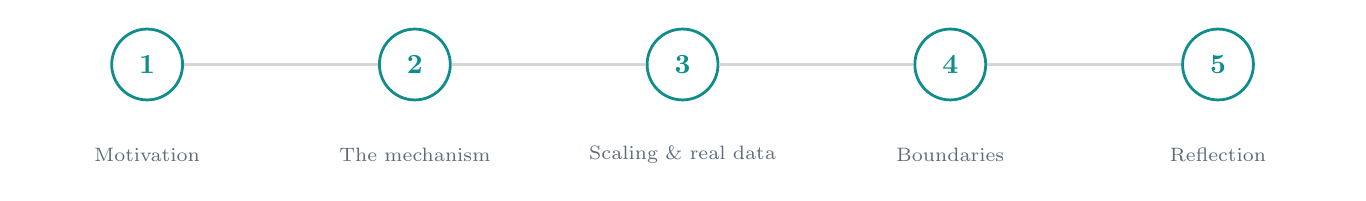
\begin{tikzpicture}[stn/.style={circle,draw=owteal,line width=1pt,minimum size=9mm,font=\bfseries,inner sep=0,text=owteal},std/.style={circle,draw=owteal,fill=owteal,line width=1pt,minimum size=9mm,font=\bfseries,inner sep=0,text=white},stc/.style={circle,draw=owochre,fill=owochre,line width=1.2pt,minimum size=11.5mm,font=\bfseries,inner sep=0,text=white},stx/.style={circle,draw=owmuted,line width=1pt,minimum size=9mm,font=\bfseries,inner sep=0,text=owmuted},stlbl/.style={font=\scriptsize,text=owmuted,align=center,text width=28mm},stln/.style={draw=black!16,line width=1.4pt}]\node[stn] (s0) at (0.0,0) {1};\node[stn] (s1) at (3.4,0) {2};\node[stn] (s2) at (6.8,0) {3};\node[stn] (s3) at (10.2,0) {4};\node[stn] (s4) at (13.6,0) {5};\node[stlbl] at (0.0,-1.15) {Motivation};\node[stlbl] at (3.4,-1.15) {The mechanism};\node[stlbl] at (6.8,-1.15) {Scaling \& real data};\node[stlbl] at (10.2,-1.15) {Boundaries};\node[stlbl] at (13.6,-1.15) {Reflection};\draw[stln] (s0)--(s1);\draw[stln] (s1)--(s2);\draw[stln] (s2)--(s3);\draw[stln] (s3)--(s4);\end{tikzpicture}}\vfill\end{frame}
\begin{frame}[plain]\vfill\centering \resizebox{0.95\textwidth}{!}{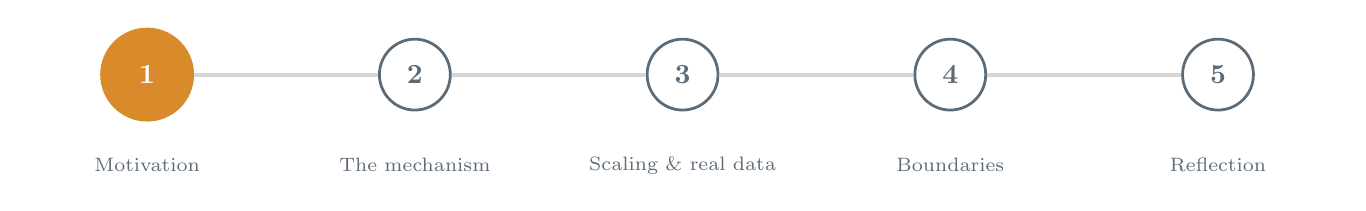
\begin{tikzpicture}[stn/.style={circle,draw=owteal,line width=1pt,minimum size=9mm,font=\bfseries,inner sep=0,text=owteal},std/.style={circle,draw=owteal,fill=owteal,line width=1pt,minimum size=9mm,font=\bfseries,inner sep=0,text=white},stc/.style={circle,draw=owochre,fill=owochre,line width=1.2pt,minimum size=11.5mm,font=\bfseries,inner sep=0,text=white},stx/.style={circle,draw=owmuted,line width=1pt,minimum size=9mm,font=\bfseries,inner sep=0,text=owmuted},stlbl/.style={font=\scriptsize,text=owmuted,align=center,text width=28mm},stln/.style={draw=black!16,line width=1.4pt}]\node[stc] (s0) at (0.0,0) {1};\node[stx] (s1) at (3.4,0) {2};\node[stx] (s2) at (6.8,0) {3};\node[stx] (s3) at (10.2,0) {4};\node[stx] (s4) at (13.6,0) {5};\node[stlbl] at (0.0,-1.15) {Motivation};\node[stlbl] at (3.4,-1.15) {The mechanism};\node[stlbl] at (6.8,-1.15) {Scaling \& real data};\node[stlbl] at (10.2,-1.15) {Boundaries};\node[stlbl] at (13.6,-1.15) {Reflection};\draw[stln] (s0)--(s1);\draw[stln] (s1)--(s2);\draw[stln] (s2)--(s3);\draw[stln] (s3)--(s4);\end{tikzpicture}}\\[24pt]
{\color{owochre}\bfseries\footnotesize PART 1}\\[5pt]
{\color{owdeep}\bfseries\Large Motivation}\\[10pt]{\color{owmuted}\large Manufacturing experience}\vfill\end{frame}
\begin{frame}{The problem: experience is scarce}
\begin{itemize}
  \item LLMs generalize only after many real, labeled examples
  \item In most domains that experience is scarce and costly
  \item We study a way to manufacture it cheaply
  \item Idea: when dynamics can be written as code, simulate the experience
\end{itemize}
\end{frame}
\begin{frame}{Two species of world model}
\begin{itemize}
  \item Perceptual/generative: learned nets, latents/pixels/video (Dreamer, Genie, Sora)
  \item Data-hungry, compounding error, opaque weights
  \item Code World Models (CWMs): transition is a readable program over symbolic state
  \item Synthesized by an LLM, verified before use, exact rollouts, zero training data
\end{itemize}
\end{frame}
\begin{frame}[plain]\centering\vfill
{\color{owdeep}\bfseries\LARGE Where spatial-intelligence systems learn what cannot be told, OpenWorld writes down what can be told -- and verifies it.\par}\vfill\end{frame}
\begin{frame}{Two conditions make it work}
\begin{itemize}
  \item Worlds must not lie: dynamics are verified code, not learned approximations
  \item Accepted only if it parses, runs sandboxed, preserves invariants, survives a critic
  \item Need many worlds -- each must be cheap to build
  \item OpenWorld makes authoring a verified world a minutes-scale activity
\end{itemize}
\end{frame}
\begin{frame}{Contributions}
\begin{itemize}
  \item World-time compute on real domains, with cross-world transfer
  \item Why it must be verified code: exact rollouts, no compounding error
  \item OpenWorld substrate + full reproducibility (79 experiments, seed-fixed)
\end{itemize}
\end{frame}
\begin{frame}[plain]\centering\vfill
{\color{owochre}\rule{40pt}{2.5pt}}\par\vskip10pt
{\color{owdeep}\bfseries\Large Problem Setting\par}\vfill\end{frame}
\begin{frame}{Symbolic-state worlds}
\begin{itemize}
  \item State is JSON-serializable; actions discrete; dynamics declarable as rules
  \item Covers triage, negotiation, portfolios, sprints, program repair
  \item Not pixel-native domains -- that is the scope boundary
  \item The adversary is model error: hallucinated transitions, silently wrong code
\end{itemize}
\end{frame}
\begin{frame}{A world model, formally}
\begin{itemize}
  \item W = (states, actions, s0, transition tau, weighted objectives, invariants)
  \item Practitioner declares everything but tau (schema, actions, rules, dials)
  \item Framework produces tau by synthesis under verification, not learning
  \item Certifies invariant-consistency, not equality to true dynamics
\end{itemize}
\end{frame}
\begin{frame}{Verified code is exact at every depth}\centering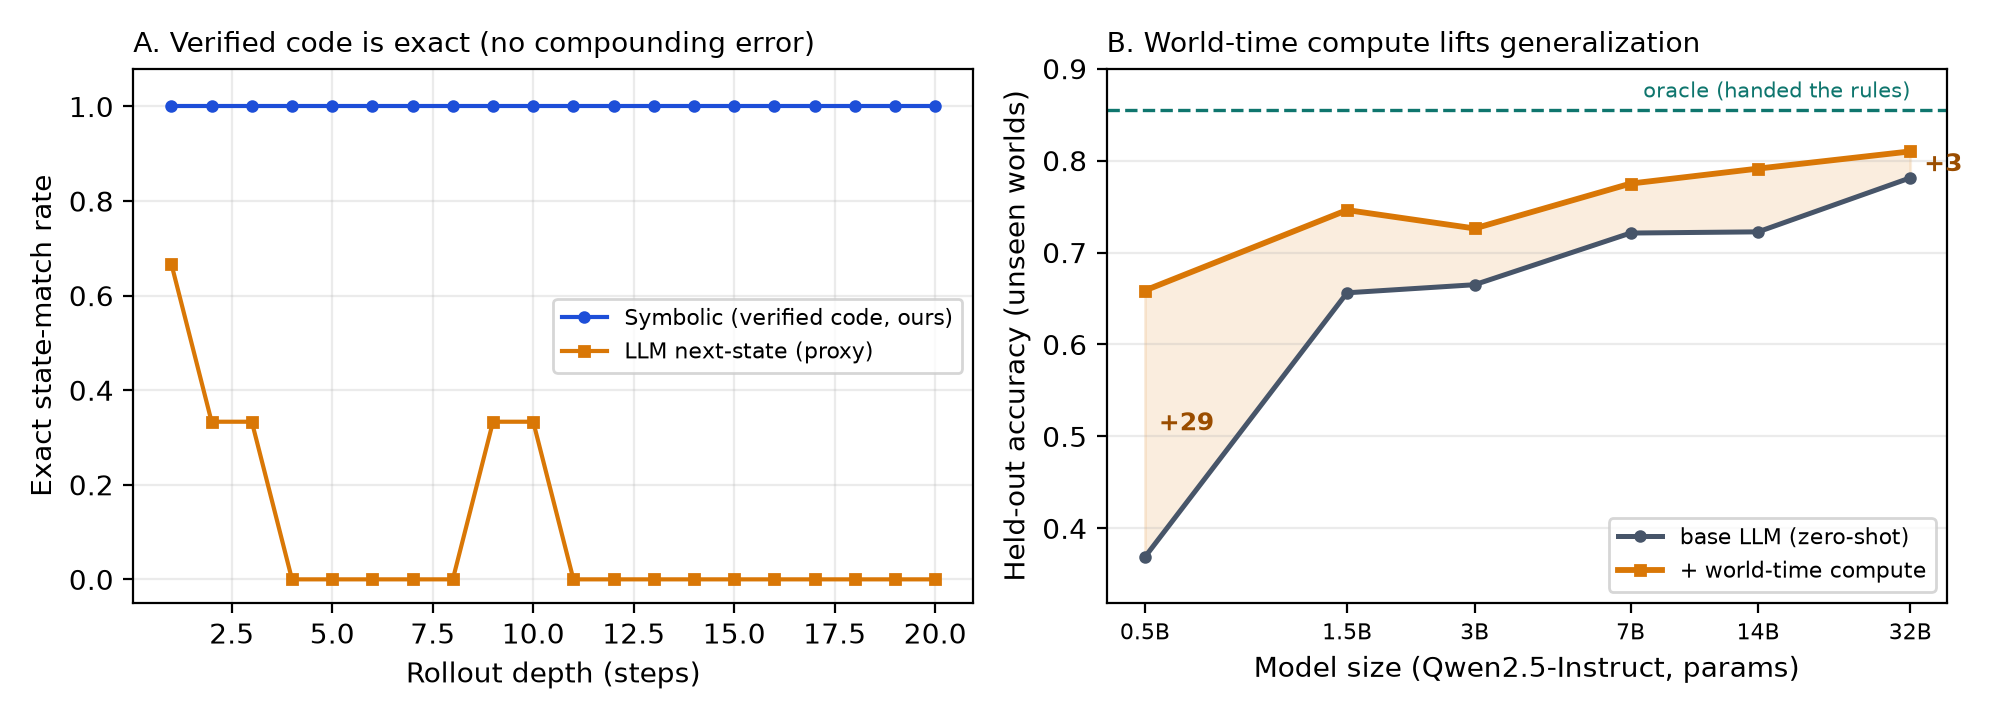
\includegraphics[width=\linewidth,height=0.74\textheight,keepaspectratio]{hero.png}\end{frame}
\begin{frame}[plain]\centering\vfill
{\color{owochre}\rule{40pt}{2.5pt}}\par\vskip10pt
{\color{owdeep}\bfseries\Large Method \& Experimental Setup\par}\vfill\end{frame}
\begin{frame}{Worlds and models}
\begin{itemize}
  \item Three oracle worlds: sprint, orchard, triage (hand-written ground truth)
  \item Coding world: 20 buggy-function repair tasks, transition = test execution
  \item Local Ollama models: qwen2.5 1.5B/3B/7B, plus Llama-3.1-8B, Gemma2-9B
  \item Fine-tuning runs: single cloud A100, 4-bit QLoRA
\end{itemize}
\end{frame}
\begin{frame}{Baselines and metrics}
\begin{itemize}
  \item LLMTransition: same backbone predicting each next state (learned-style proxy)
  \item Trained MLP + 1-NN on K = 100 / 1k / 10k random transitions
  \item Exact-state match, first-divergence step, final L1 error; pass@k for repair
  \item 95\% Wilson CIs; every number regenerates from one script
\end{itemize}
\end{frame}
\begin{frame}[plain]\vfill\centering \resizebox{0.95\textwidth}{!}{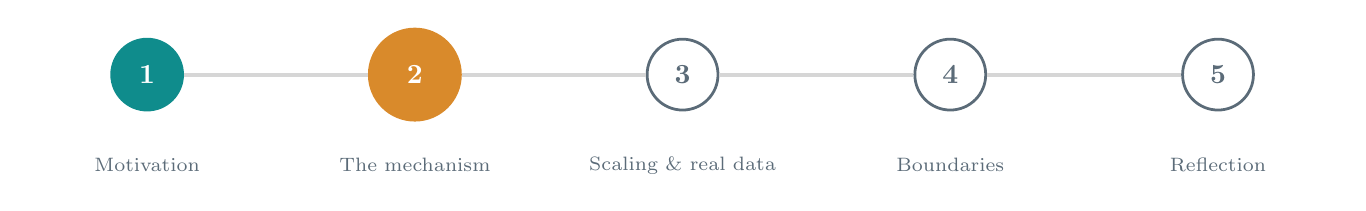
\begin{tikzpicture}[stn/.style={circle,draw=owteal,line width=1pt,minimum size=9mm,font=\bfseries,inner sep=0,text=owteal},std/.style={circle,draw=owteal,fill=owteal,line width=1pt,minimum size=9mm,font=\bfseries,inner sep=0,text=white},stc/.style={circle,draw=owochre,fill=owochre,line width=1.2pt,minimum size=11.5mm,font=\bfseries,inner sep=0,text=white},stx/.style={circle,draw=owmuted,line width=1pt,minimum size=9mm,font=\bfseries,inner sep=0,text=owmuted},stlbl/.style={font=\scriptsize,text=owmuted,align=center,text width=28mm},stln/.style={draw=black!16,line width=1.4pt}]\node[std] (s0) at (0.0,0) {1};\node[stc] (s1) at (3.4,0) {2};\node[stx] (s2) at (6.8,0) {3};\node[stx] (s3) at (10.2,0) {4};\node[stx] (s4) at (13.6,0) {5};\node[stlbl] at (0.0,-1.15) {Motivation};\node[stlbl] at (3.4,-1.15) {The mechanism};\node[stlbl] at (6.8,-1.15) {Scaling \& real data};\node[stlbl] at (10.2,-1.15) {Boundaries};\node[stlbl] at (13.6,-1.15) {Reflection};\draw[stln] (s0)--(s1);\draw[stln] (s1)--(s2);\draw[stln] (s2)--(s3);\draw[stln] (s3)--(s4);\end{tikzpicture}}\\[24pt]
{\color{owochre}\bfseries\footnotesize PART 2}\\[5pt]
{\color{owdeep}\bfseries\Large The mechanism}\\[10pt]{\color{owmuted}\large Verified code + world-time compute}\vfill\end{frame}
\begin{frame}{World-time compute, in three numbers}\vfill\begin{columns}[c]\begin{column}{0.323\textwidth}\centering{\color{owdeep}\fontsize{40}{44}\selectfont\bfseries 24/24}\\[6pt]{\color{owmuted}\small exact rollouts (code)}\end{column}\begin{column}{0.323\textwidth}\centering{\color{owdeep}\fontsize{40}{44}\selectfont\bfseries 0/24}\\[6pt]{\color{owmuted}\small exact rollouts (LLM)}\end{column}\begin{column}{0.323\textwidth}\centering{\color{owochre}\fontsize{40}{44}\selectfont\bfseries +29 pts}\\[6pt]{\color{owmuted}\small held-out lift at 0.5B}\end{column}\end{columns}\vfill\end{frame}
\begin{frame}{Verified code eliminates compounding error}
\centering
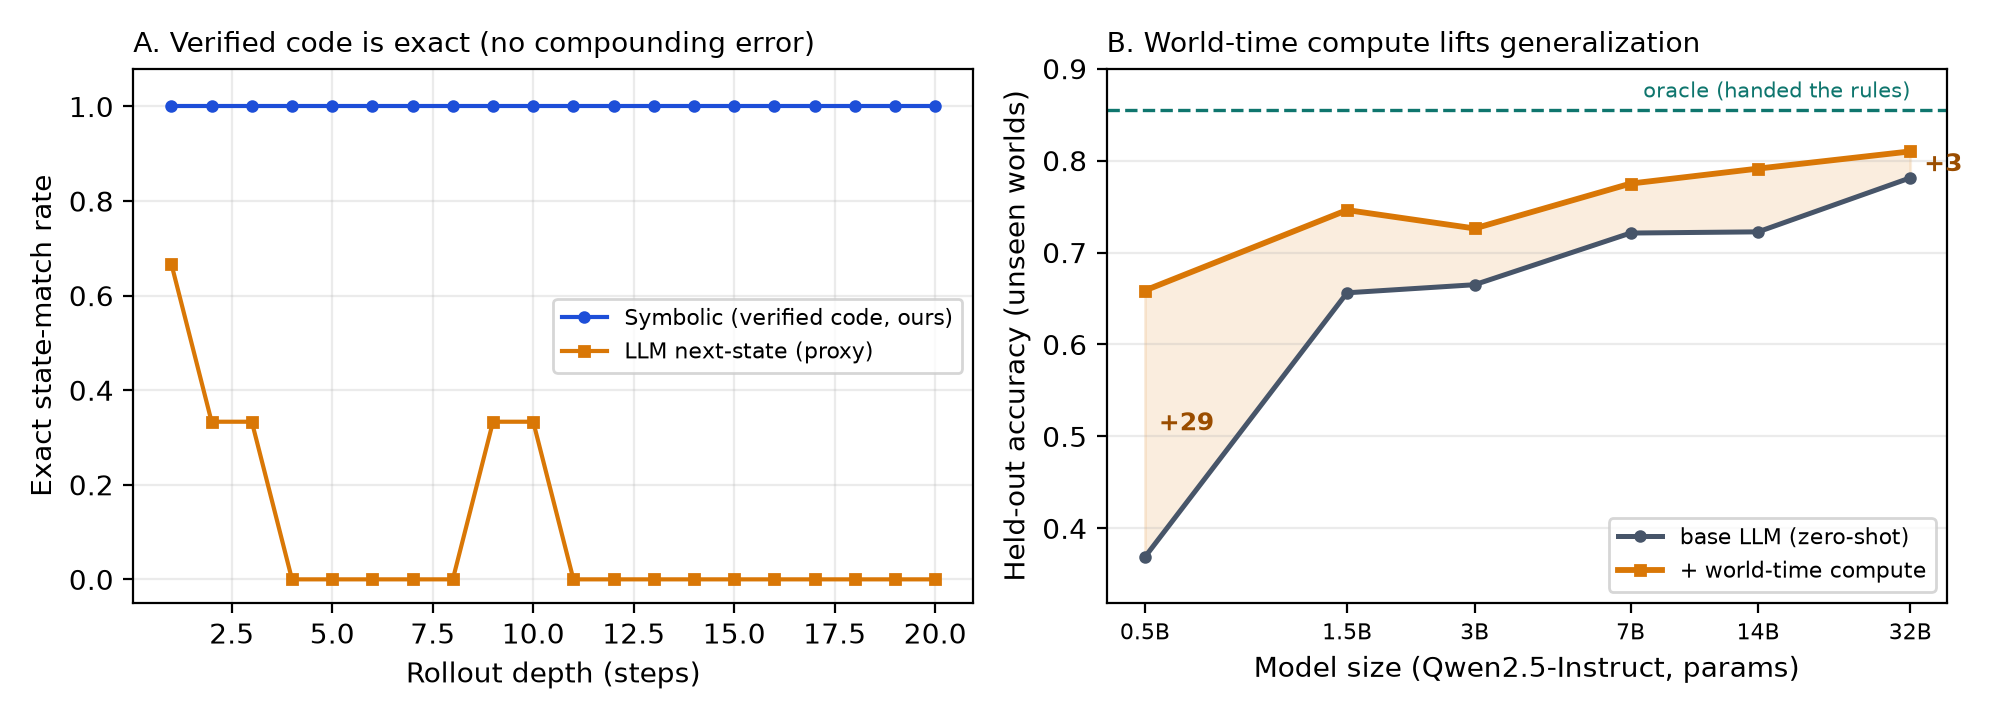
\includegraphics[width=\linewidth,height=0.48\textheight,keepaspectratio]{hero.png}\vskip3pt{\color{owmuted}\footnotesize A: code exact at every depth vs LLM diverging by step \textasciitilde{}2.3. B: world-time compute payoff.\par}
\flushleft \vskip3pt{\footnotesize \begin{itemize}
  \item Code (blue) matches oracle exactly across a 20-step rollout
  \item Per-step LLM (orange) first diverges \textasciitilde{}step 2.3, never completes exactly
  \item B: fine-tuning on 60 verified worlds lifts held-out accuracy
  \item Largest gain for smallest models: +29 pts at 0.5B, +3 at 32B
\end{itemize}}
\end{frame}
\begin{frame}{Head-to-head dynamics fidelity (E1/E4/E11)}
\centering
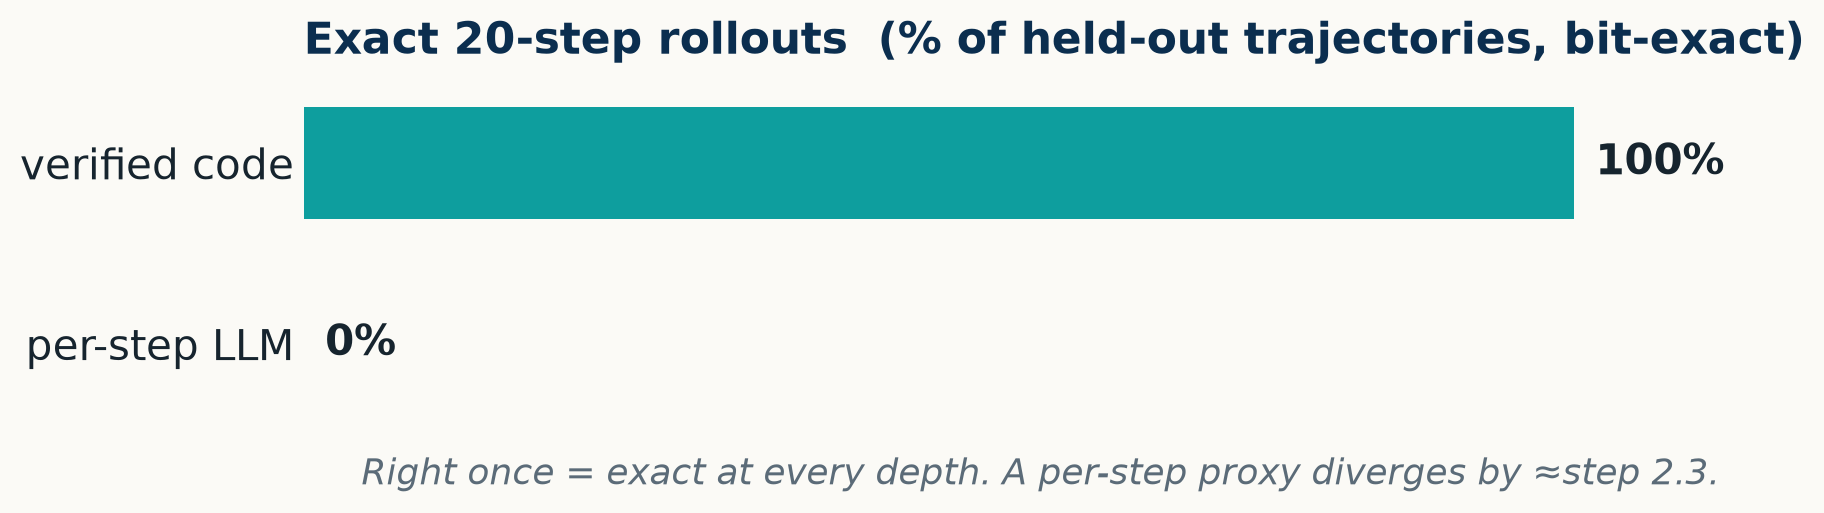
\includegraphics[width=\linewidth,height=0.48\textheight,keepaspectratio]{pres_exact.png}\vskip3pt{\color{owmuted}\footnotesize Right once = exact at every depth; the per-step proxy never completes exactly\par}
\flushleft \vskip3pt{\footnotesize \begin{itemize}
  \item Code rolls out at \textasciitilde{}15,000 steps/s vs the LLM's 0.32 steps/s
  \item OOD probes: code 100\% exact from zero transitions
\end{itemize}}
\end{frame}
\begin{frame}[plain]\centering\vfill
{\color{owdeep}\bfseries\LARGE The robust claim is the exact-match contrast, not the mean divergence step -- compounding depends on per-world error rate.\par}\vfill\end{frame}
\begin{frame}[plain]\centering\vfill
{\color{owochre}\rule{40pt}{2.5pt}}\par\vskip10pt
{\color{owdeep}\bfseries\Large World-Time Compute: Traversing Worlds to Generalize\par}\vfill\end{frame}
\begin{frame}{What world-time compute is}\centering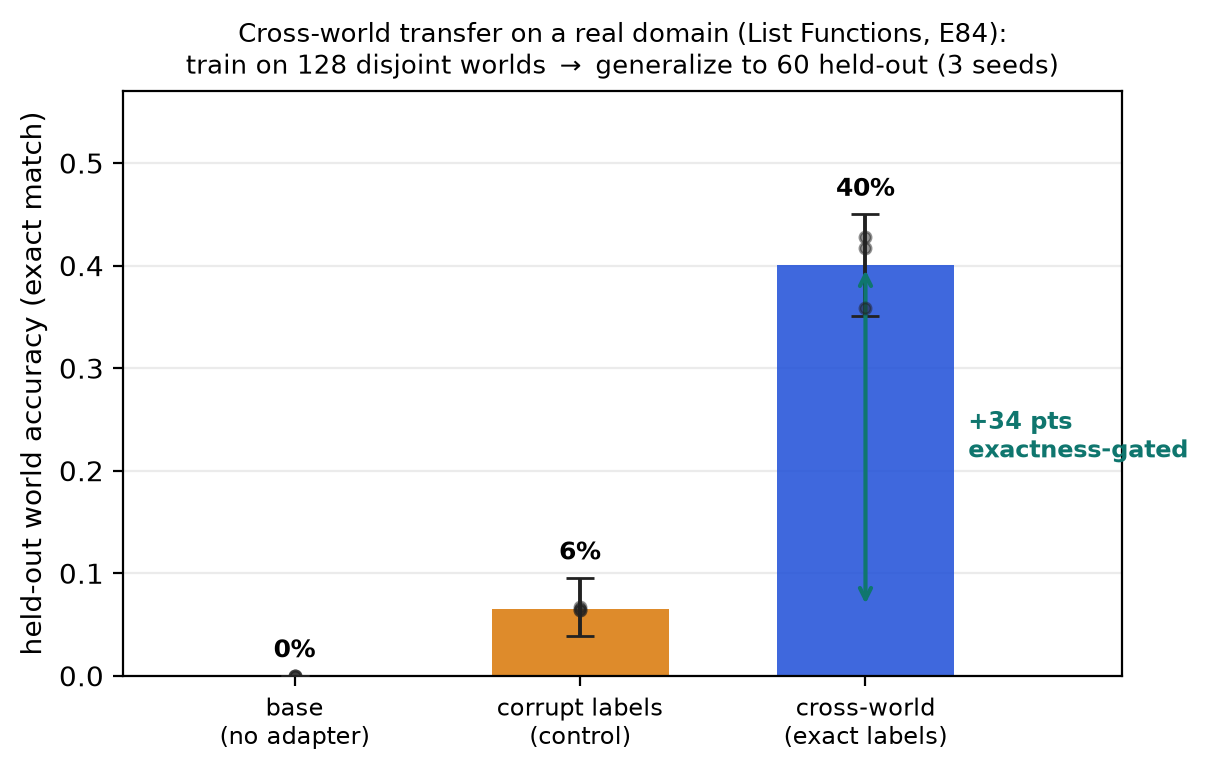
\includegraphics[width=\linewidth,height=0.74\textheight,keepaspectratio]{crossworld.png}\end{frame}
\begin{frame}{Anatomy of one diagnosis world (E74)}
\centering
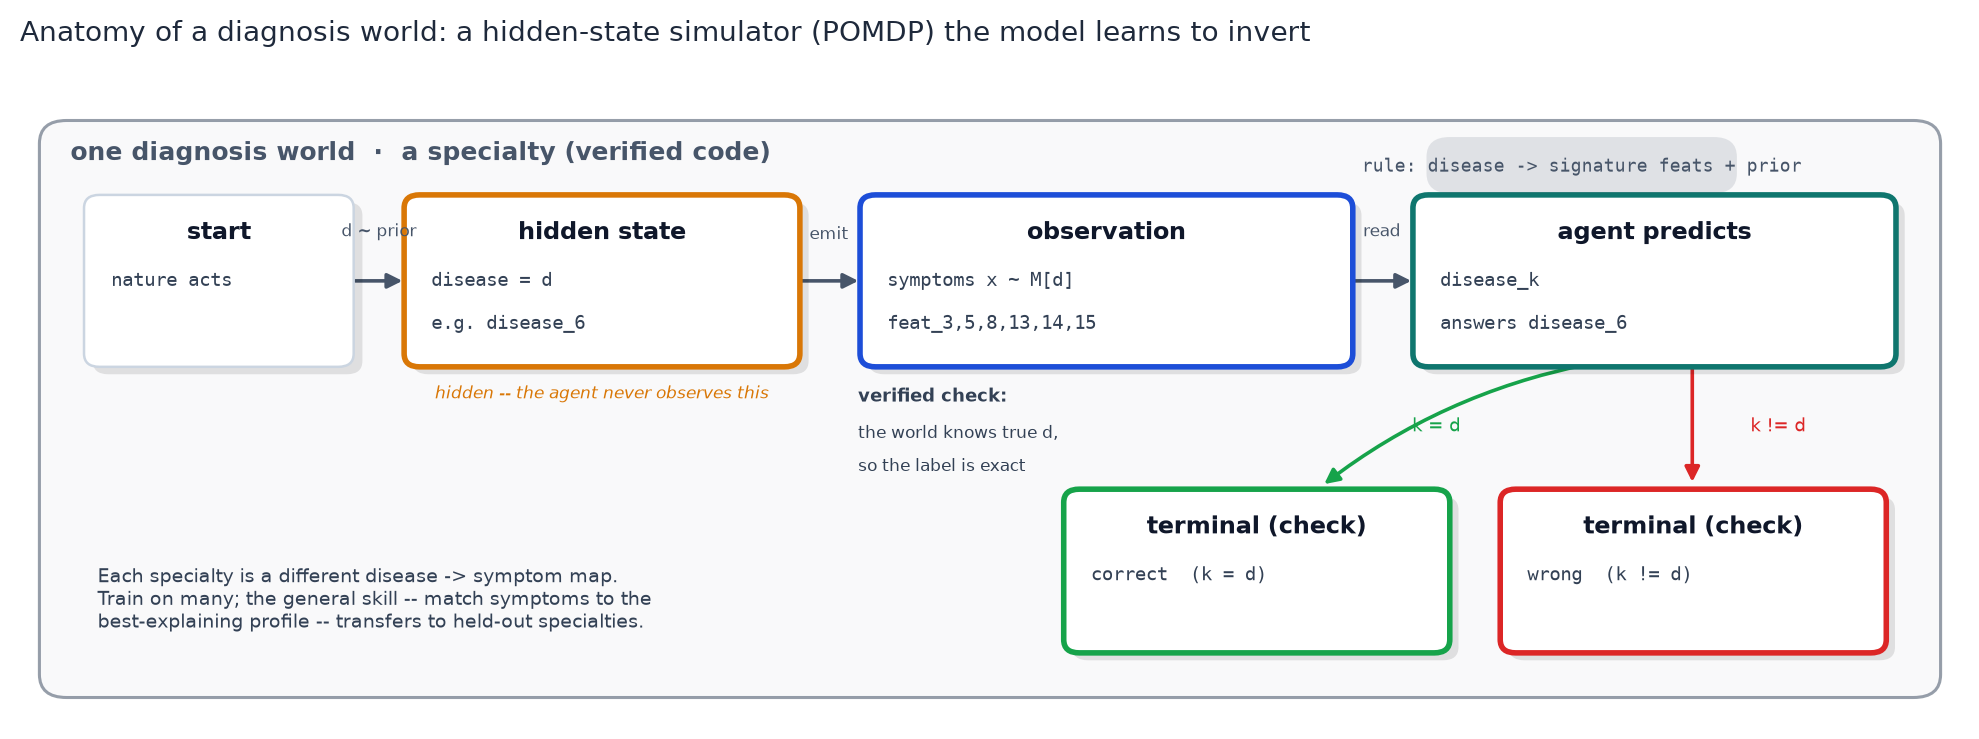
\includegraphics[width=\linewidth,height=0.48\textheight,keepaspectratio]{diagnosis_world.png}\vskip3pt{\color{owmuted}\footnotesize Hidden disease -> emitted symptoms; agent inverts observation to name the disease.\par}
\flushleft \vskip3pt{\footnotesize \begin{itemize}
  \item Each specialty is a small hidden-state simulator with a known label
  \item Agent treats its own verified world as ground truth
  \item Train on many specialties, test on held-out ones
  \item Forces the general skill, not memorization
\end{itemize}}
\end{frame}
\begin{frame}{Generalization, not memorization -- and a small-model multiplier}
\centering
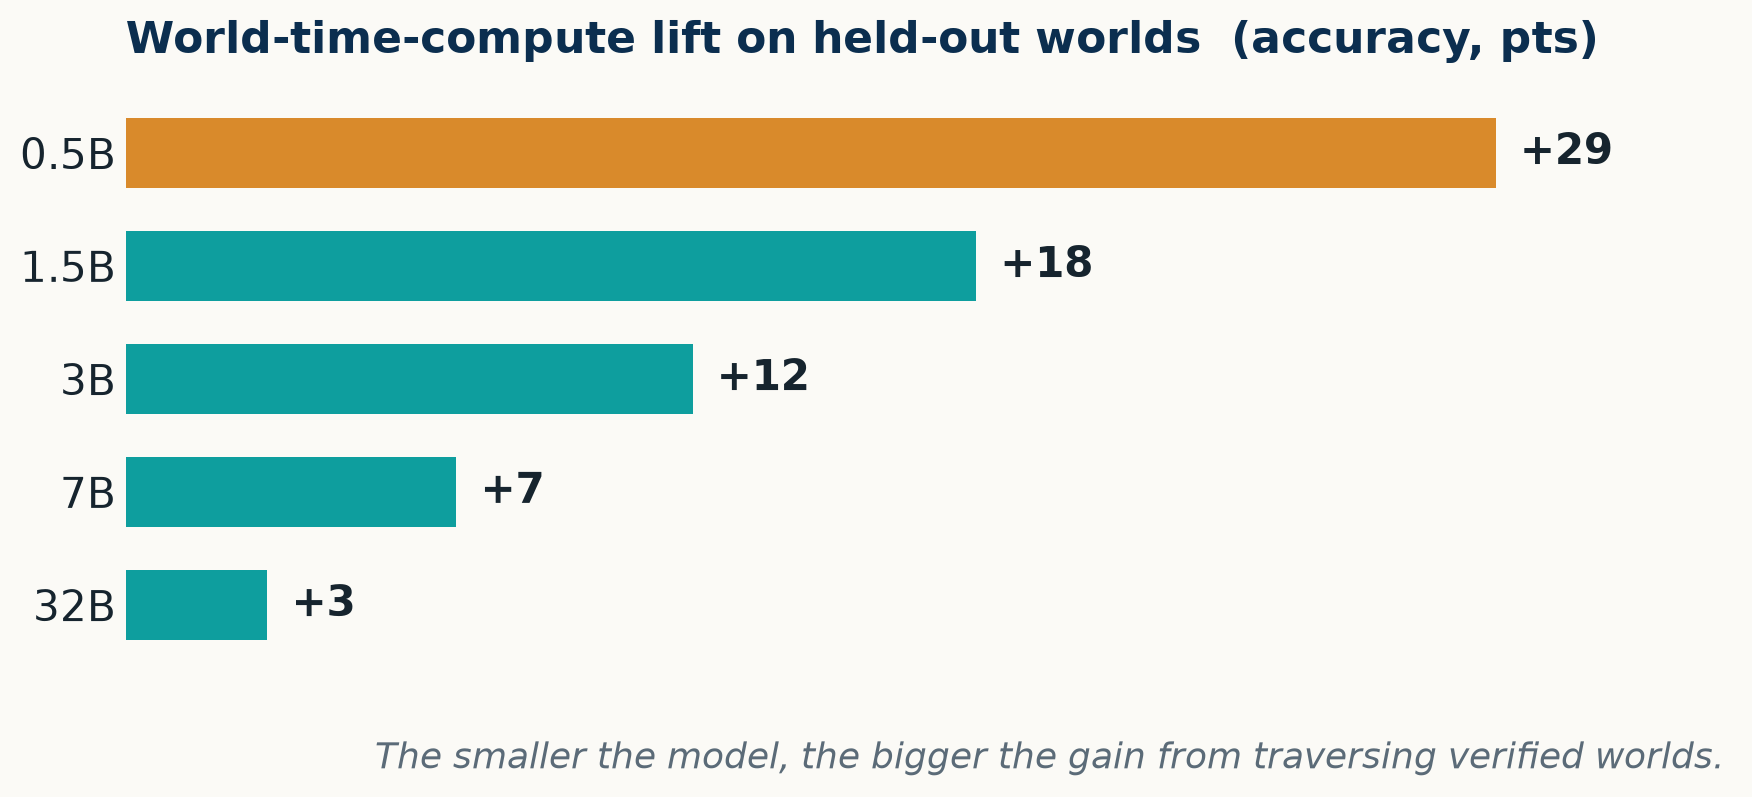
\includegraphics[width=\linewidth,height=0.48\textheight,keepaspectratio]{pres_smallmodel.png}\vskip3pt{\color{owmuted}\footnotesize Lift at every model size on unseen worlds; the smaller the model, the bigger the gain\par}
\flushleft \vskip3pt{\footnotesize \begin{itemize}
  \item 0.5B: 37\% -> 66\%; 32B: 78\% -> 81\% toward the 86\% rules-given oracle
  \item Heterogeneous worlds sharing no skill (E71/E73) give no transfer
\end{itemize}}
\end{frame}
\begin{frame}[plain]\vfill\centering \resizebox{0.95\textwidth}{!}{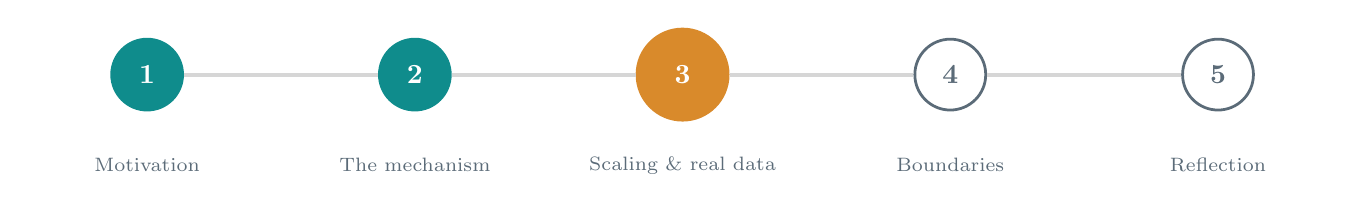
\begin{tikzpicture}[stn/.style={circle,draw=owteal,line width=1pt,minimum size=9mm,font=\bfseries,inner sep=0,text=owteal},std/.style={circle,draw=owteal,fill=owteal,line width=1pt,minimum size=9mm,font=\bfseries,inner sep=0,text=white},stc/.style={circle,draw=owochre,fill=owochre,line width=1.2pt,minimum size=11.5mm,font=\bfseries,inner sep=0,text=white},stx/.style={circle,draw=owmuted,line width=1pt,minimum size=9mm,font=\bfseries,inner sep=0,text=owmuted},stlbl/.style={font=\scriptsize,text=owmuted,align=center,text width=28mm},stln/.style={draw=black!16,line width=1.4pt}]\node[std] (s0) at (0.0,0) {1};\node[std] (s1) at (3.4,0) {2};\node[stc] (s2) at (6.8,0) {3};\node[stx] (s3) at (10.2,0) {4};\node[stx] (s4) at (13.6,0) {5};\node[stlbl] at (0.0,-1.15) {Motivation};\node[stlbl] at (3.4,-1.15) {The mechanism};\node[stlbl] at (6.8,-1.15) {Scaling \& real data};\node[stlbl] at (10.2,-1.15) {Boundaries};\node[stlbl] at (13.6,-1.15) {Reflection};\draw[stln] (s0)--(s1);\draw[stln] (s1)--(s2);\draw[stln] (s2)--(s3);\draw[stln] (s3)--(s4);\end{tikzpicture}}\\[24pt]
{\color{owochre}\bfseries\footnotesize PART 3}\\[5pt]
{\color{owdeep}\bfseries\Large Scaling \& real data}\\[10pt]{\color{owmuted}\large World-count, exact labels, real domains}\vfill\end{frame}
\begin{frame}{World-count scaling (E76)}
\centering
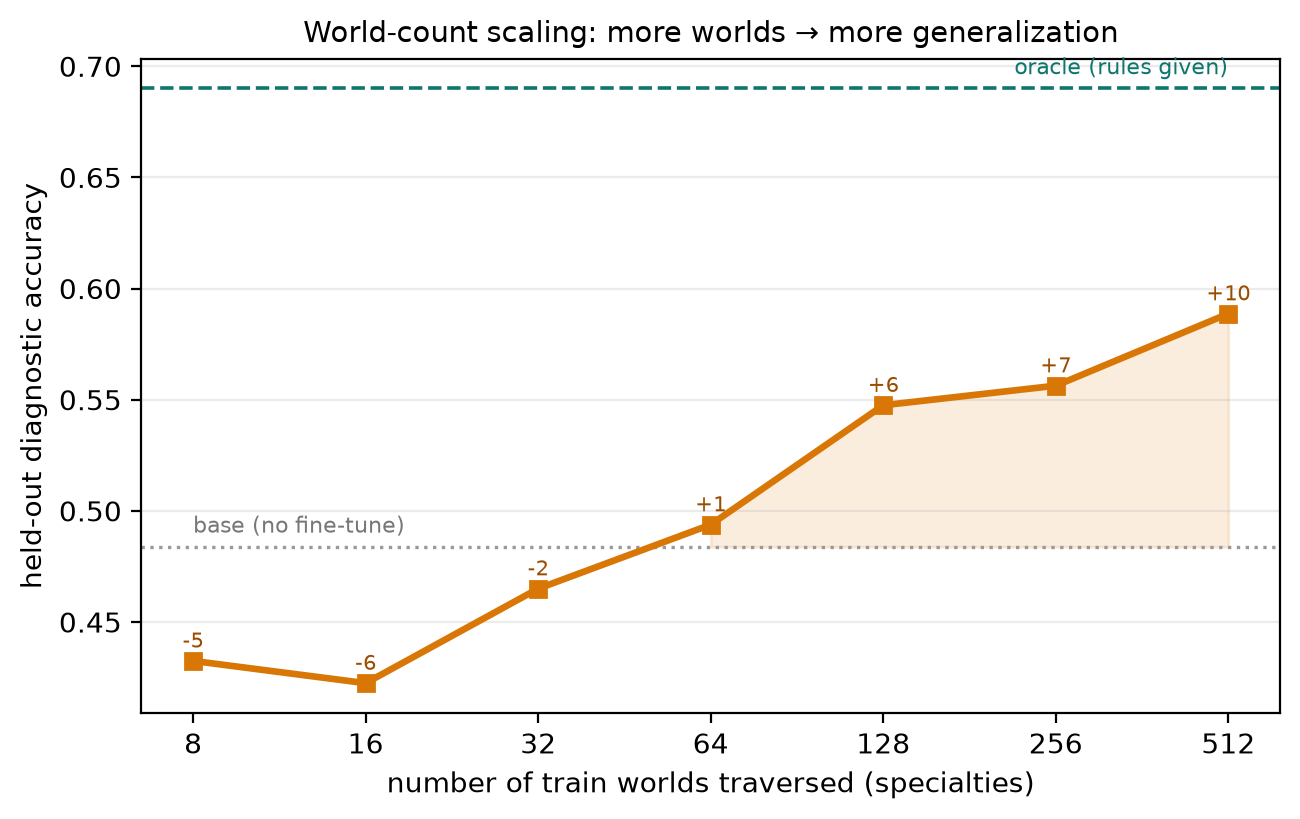
\includegraphics[width=\linewidth,height=0.48\textheight,keepaspectratio]{world_count.png}\vskip3pt{\color{owmuted}\footnotesize Held-out accuracy vs number of train worlds; still climbing at 512 worlds.\par}
\flushleft \vskip3pt{\footnotesize \begin{itemize}
  \item Too few worlds hurt (below 48\% base) -- overfits a narrow slice
  \item Gain then rises monotonically, no plateau
  \item Still climbing at 512 worlds: 59\% (+10 pts), heading toward 69\% oracle
  \item A genuine scaling lever in the number of worlds
\end{itemize}}
\end{frame}
\begin{frame}{Exact labels are the lever (E78b)}
\centering

\includegraphics[width=\linewidth,height=0.48\textheight,keepaspectratio]{noise_ablation.png}\vskip3pt{\color{owmuted}\footnotesize Corrupt a fraction p of training labels; accuracy falls monotonically.\par}
\flushleft \vskip3pt{\footnotesize \begin{itemize}
  \item 256 worlds fixed; only training labels corrupted at rate p
  \item Verified (p=0): 35\%; fully wrong (p=1): 19\%, at/below floor
  \item Label exactness -- not task variety -- drives the effect
  \item This is what separates world-time compute from domain randomization
\end{itemize}}
\end{frame}
\begin{frame}{A coding-world family (E77)}
\begin{itemize}
  \item 164 function-implementation worlds, each verified by its pytest oracle
  \item In-domain: 7B pass@5 lifts 84\% -> 95\% at every size
  \item HumanEval (OOD): hurts greedy pass@1 (78\% -> 70\%)
  \item But transfers positively at pass@5 (87\% -> 91\%) from only 164 worlds
\end{itemize}
\end{frame}
\begin{frame}[plain]\centering\vfill
{\color{owochre}\rule{40pt}{2.5pt}}\par\vskip10pt
{\color{owdeep}\bfseries\Large Real Data: World-Time Compute on ARC-AGI\par}\vfill\end{frame}
\begin{frame}{How WTC fine-tunes on a verified world (E80)}
\centering
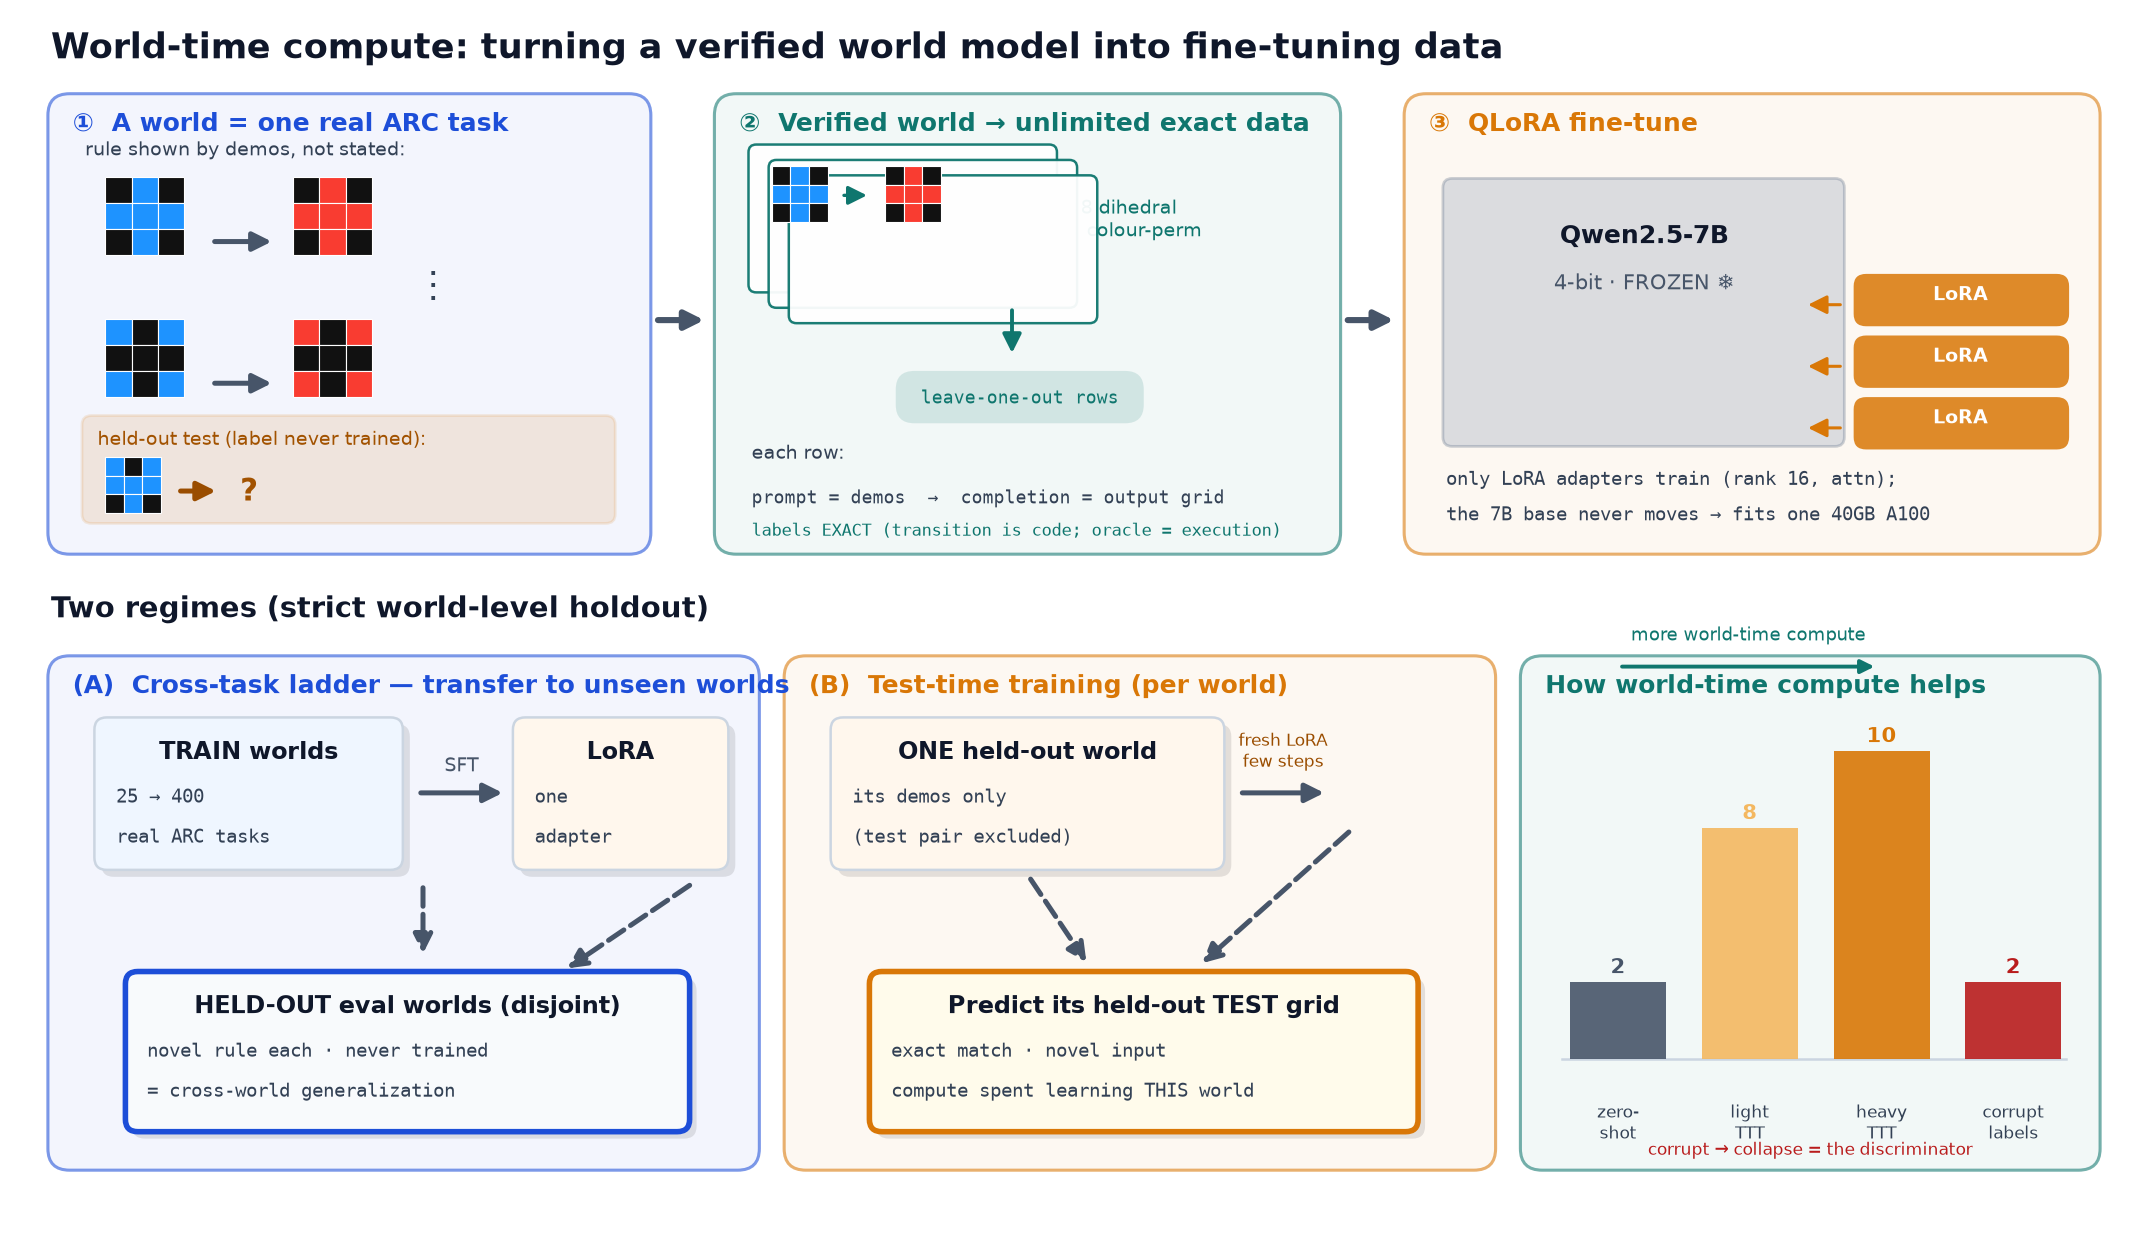
\includegraphics[width=\linewidth,height=0.48\textheight,keepaspectratio]{arc_method.png}\vskip3pt{\color{owmuted}\footnotesize ARC task -> augmented exactly-labeled rows -> QLoRA on frozen 4-bit Qwen2.5-7B.\par}
\flushleft \vskip3pt{\footnotesize \begin{itemize}
  \item Each ARC task is a world with a latent rule shown by demonstrations
  \item Rule-preserving augmentation (dihedral x color) -> unlimited labeled rows
  \item Two strict holdouts: cross-task ladder and per-world test-time training
  \item Corrupted-label arm is the discriminator
\end{itemize}}
\end{frame}
\begin{frame}{World-time compute on real ARC-AGI (E80)}
\centering
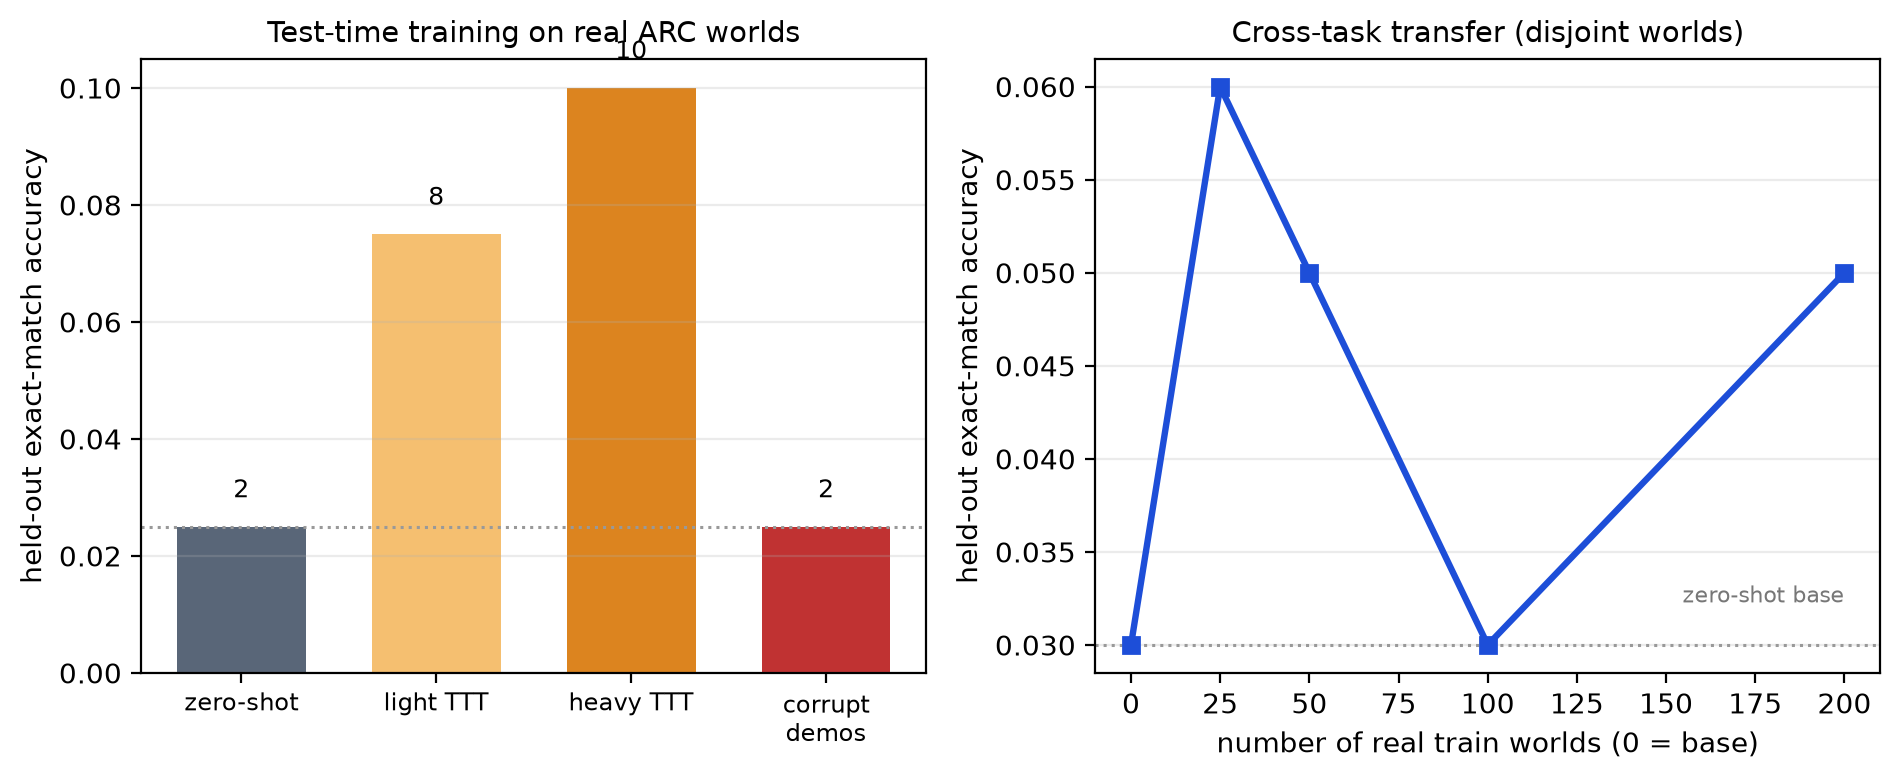
\includegraphics[width=\linewidth,height=0.48\textheight,keepaspectratio]{arc.png}\vskip3pt{\color{owmuted}\footnotesize Per-world TTT lifts exact-match; cross-task transfer stays weak.\par}
\flushleft \vskip3pt{\footnotesize \begin{itemize}
  \item Zero-shot 2\% -> light 8\% -> heavy 10\% (+8 pts) with more compute
  \item Corrupted demos fall to 2\%, at the zero-shot floor
  \item Lift requires verified labels -- the model learns each real rule
  \item Cross-task transfer weak (3\% -> 5\%): every ARC rule is novel
\end{itemize}}
\end{frame}
\begin{frame}{Across real domains and modalities (E80)}
\centering
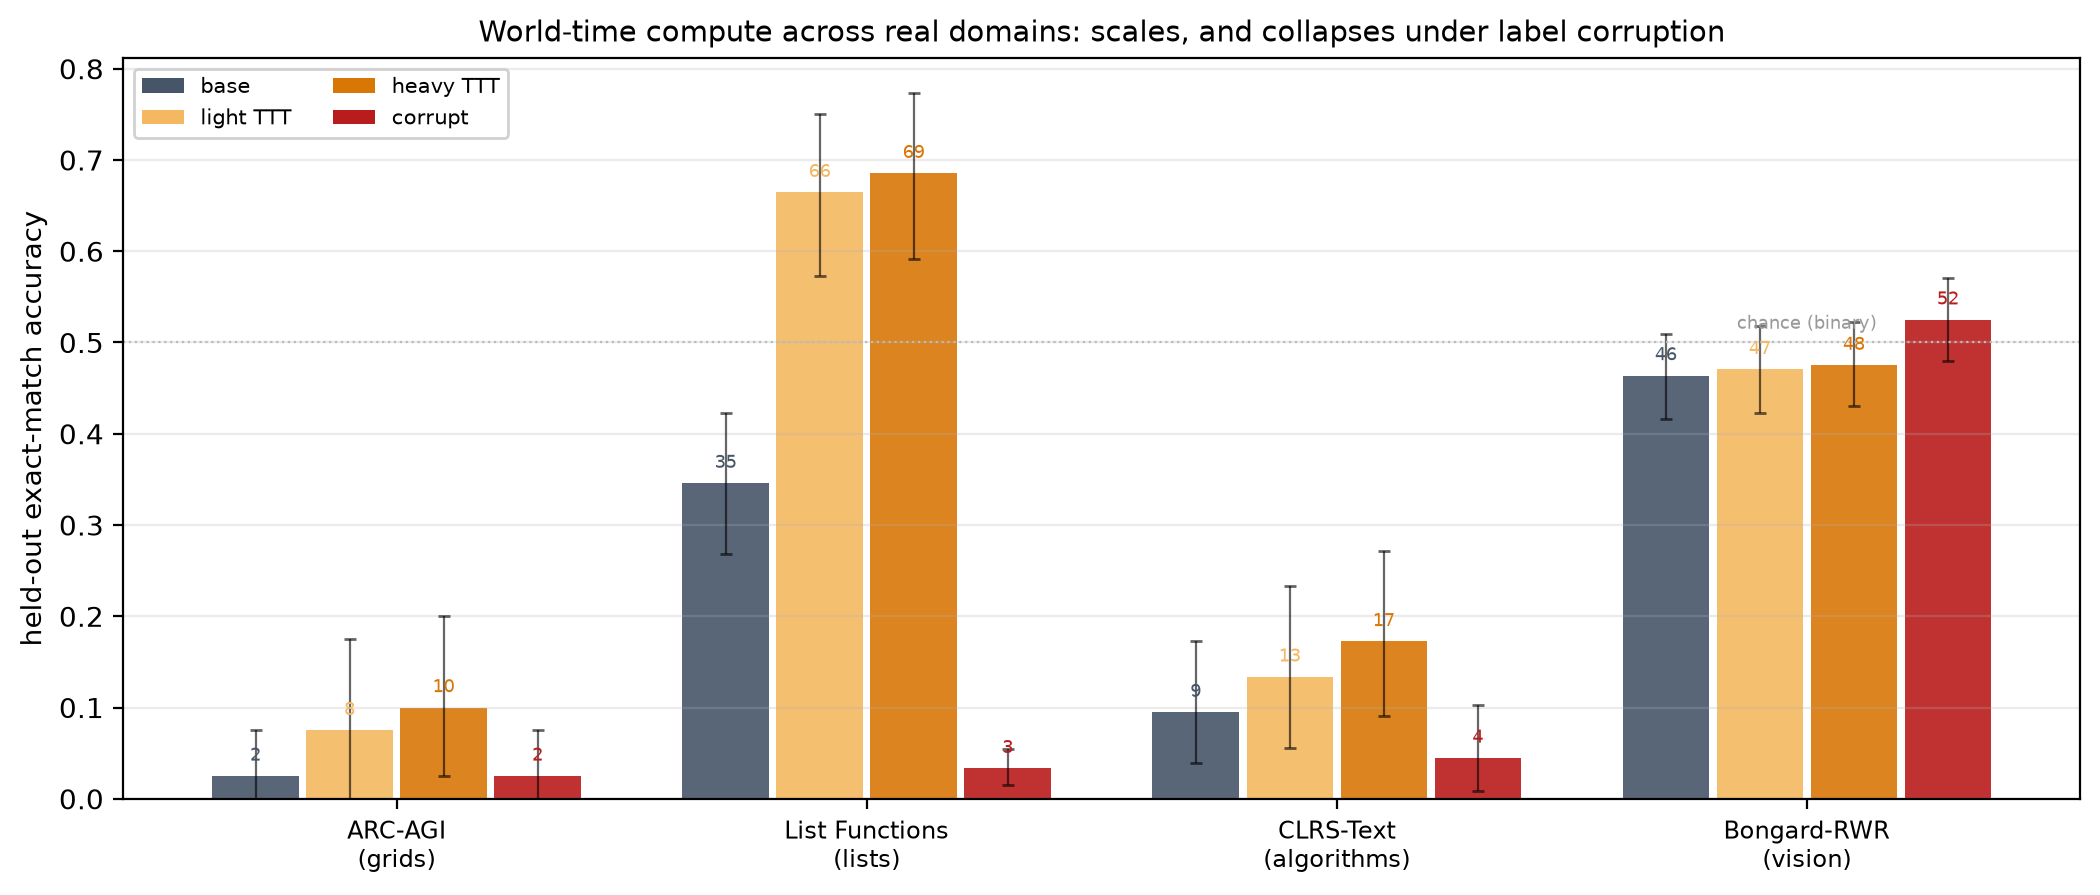
\includegraphics[width=\linewidth,height=0.48\textheight,keepaspectratio]{worldtime_domains.png}\vskip3pt{\color{owmuted}\footnotesize Scales and collapses on symbolic domains; Bongard vision stays at chance.\par}
\flushleft \vskip3pt{\footnotesize \begin{itemize}
  \item List Functions: 35\% -> 66\% -> 69\% (heavy); corrupt 3\%
  \item CLRS algorithms: 9\% -> 13\% -> 17\%; corrupt 4\%
  \item Effect largest for shallow rules, smallest for long algorithm traces
  \item Bongard-RWR (vision): flat at chance (46/48/52\%) -- the perceptual boundary
\end{itemize}}
\end{frame}
\begin{frame}[plain]\centering\vfill
{\color{owochre}\rule{40pt}{2.5pt}}\par\vskip10pt
{\color{owdeep}\bfseries\Large Cross-World Transfer on a Real Domain\par}\vfill\end{frame}
\begin{frame}{Cross-world transfer, List Functions (E84)}
\centering
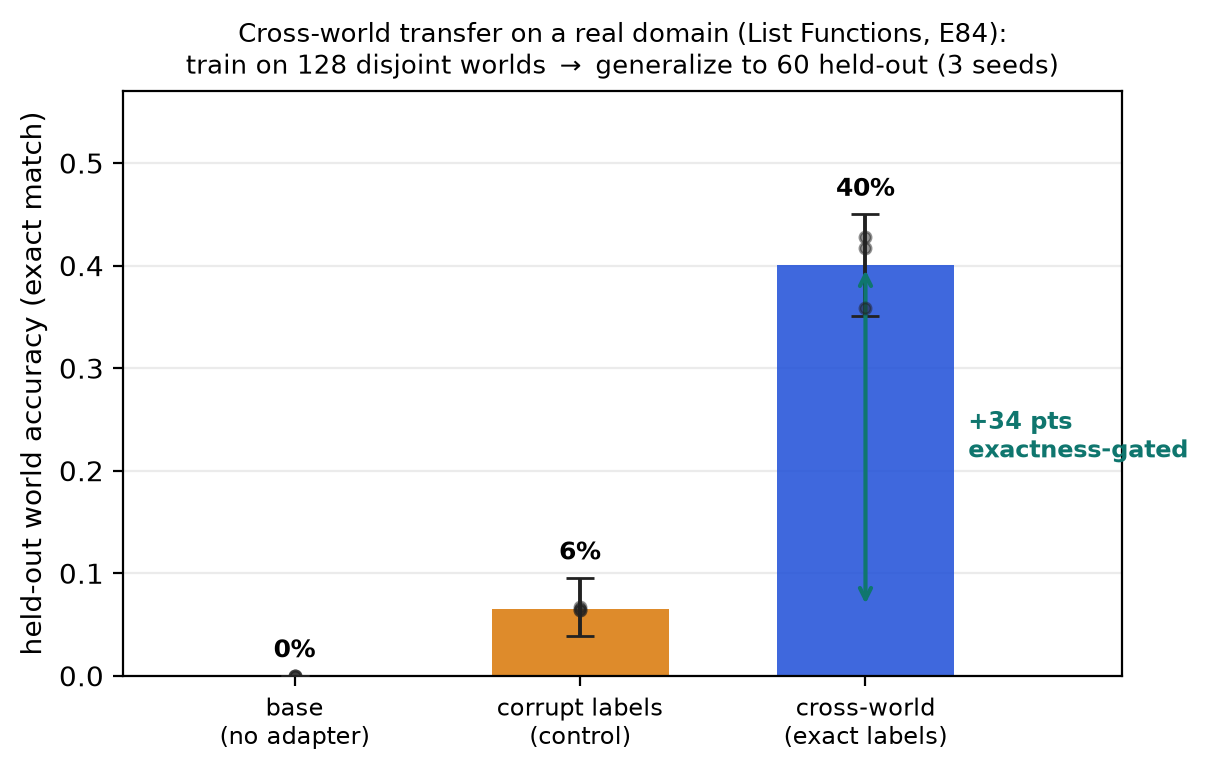
\includegraphics[width=\linewidth,height=0.48\textheight,keepaspectratio]{crossworld.png}\vskip3pt{\color{owmuted}\footnotesize One adapter on 128 disjoint worlds generalizes to 60 held-out worlds.\par}
\flushleft \vskip3pt{\footnotesize \begin{itemize}
  \item Cross-world 40\% (CI [35,45]) on worlds never seen
  \item Corrupted-label control only 6\% -- a +34-pt exactness-gated lift
  \item Gap is rule-induction transferring across worlds, not formatting
  \item The novel axis, demonstrated on data we did not generate
\end{itemize}}
\end{frame}
\begin{frame}{Cross-world transfer scales with \#worlds (E84)}
\centering
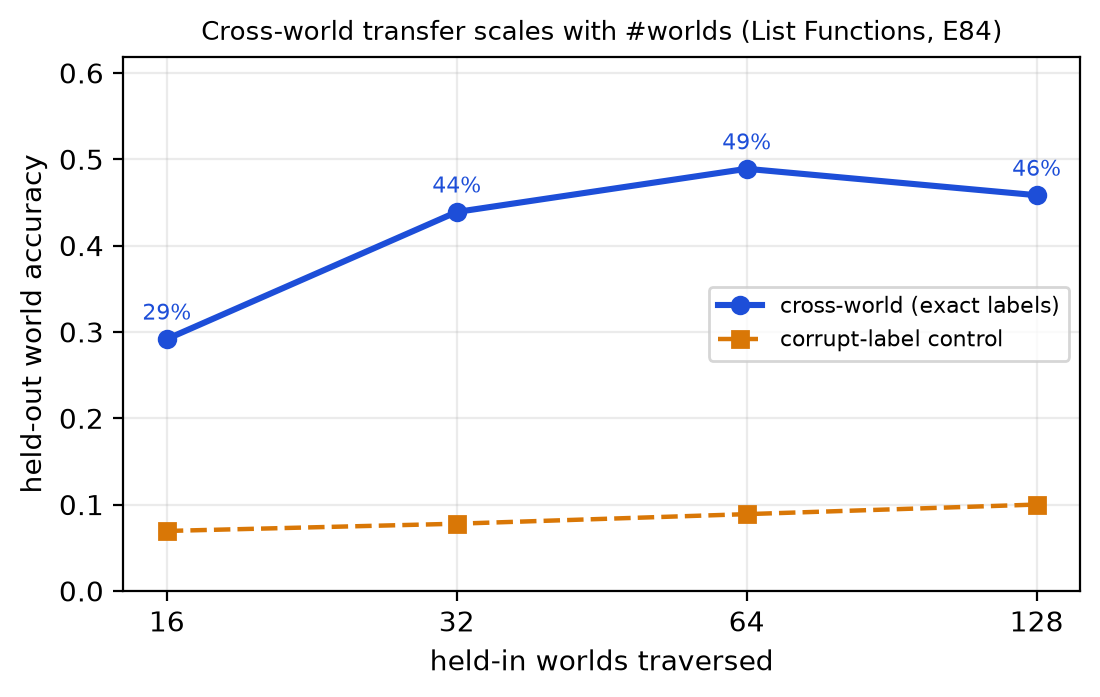
\includegraphics[width=\linewidth,height=0.48\textheight,keepaspectratio]{crossworld_ladder.png}\vskip3pt{\color{owmuted}\footnotesize Held-out accuracy 29\% -> 49\% rising then plateauing near 64 worlds.\par}
\flushleft \vskip3pt{\footnotesize \begin{itemize}
  \item Rises from 29\% at 16 worlds to a 49\% peak by 64 worlds
  \item Corrupted-label control stays flat
  \item A rising-then-plateauing scaling curve on real data
  \item More verified worlds -> more transfer
\end{itemize}}
\end{frame}
\begin{frame}{A descriptive regularity (E80)}
\begin{itemize}
  \item Saturating learning curve: acc(c) = base + (C-base)(1 - e\textasciicircum{}{-c/kappa})
  \item Asymptote tracks identifiability x realizability x headroom
  \item Light-dose probe predicts heavy asymptote (Spearman 0.73-0.98)
  \item Holds for a non-neural program synthesizer too (learner-invariance)
  \item N90 worlds: List Functions 3, ARC 9, CLRS 15 -- harder needs more
\end{itemize}
\end{frame}
\begin{frame}[plain]\vfill\centering \resizebox{0.95\textwidth}{!}{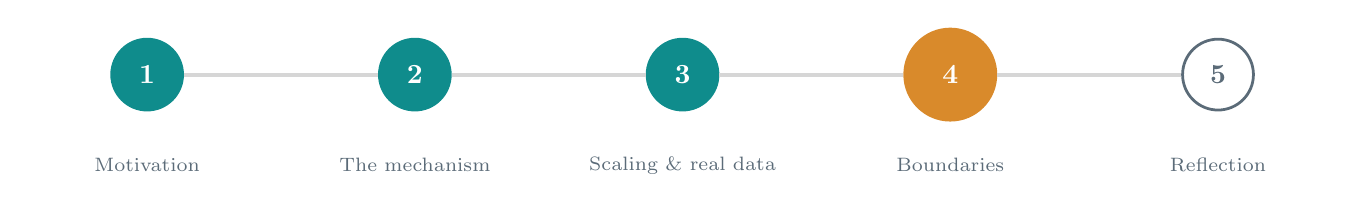
\begin{tikzpicture}[stn/.style={circle,draw=owteal,line width=1pt,minimum size=9mm,font=\bfseries,inner sep=0,text=owteal},std/.style={circle,draw=owteal,fill=owteal,line width=1pt,minimum size=9mm,font=\bfseries,inner sep=0,text=white},stc/.style={circle,draw=owochre,fill=owochre,line width=1.2pt,minimum size=11.5mm,font=\bfseries,inner sep=0,text=white},stx/.style={circle,draw=owmuted,line width=1pt,minimum size=9mm,font=\bfseries,inner sep=0,text=owmuted},stlbl/.style={font=\scriptsize,text=owmuted,align=center,text width=28mm},stln/.style={draw=black!16,line width=1.4pt}]\node[std] (s0) at (0.0,0) {1};\node[std] (s1) at (3.4,0) {2};\node[std] (s2) at (6.8,0) {3};\node[stc] (s3) at (10.2,0) {4};\node[stx] (s4) at (13.6,0) {5};\node[stlbl] at (0.0,-1.15) {Motivation};\node[stlbl] at (3.4,-1.15) {The mechanism};\node[stlbl] at (6.8,-1.15) {Scaling \& real data};\node[stlbl] at (10.2,-1.15) {Boundaries};\node[stlbl] at (13.6,-1.15) {Reflection};\draw[stln] (s0)--(s1);\draw[stln] (s1)--(s2);\draw[stln] (s2)--(s3);\draw[stln] (s3)--(s4);\end{tikzpicture}}\\[24pt]
{\color{owochre}\bfseries\footnotesize PART 4}\\[5pt]
{\color{owdeep}\bfseries\Large Boundaries}\\[10pt]{\color{owmuted}\large Where it stops working, and why}\vfill\end{frame}
\begin{frame}{Frame-invariance is a negative (E81)}
\centering
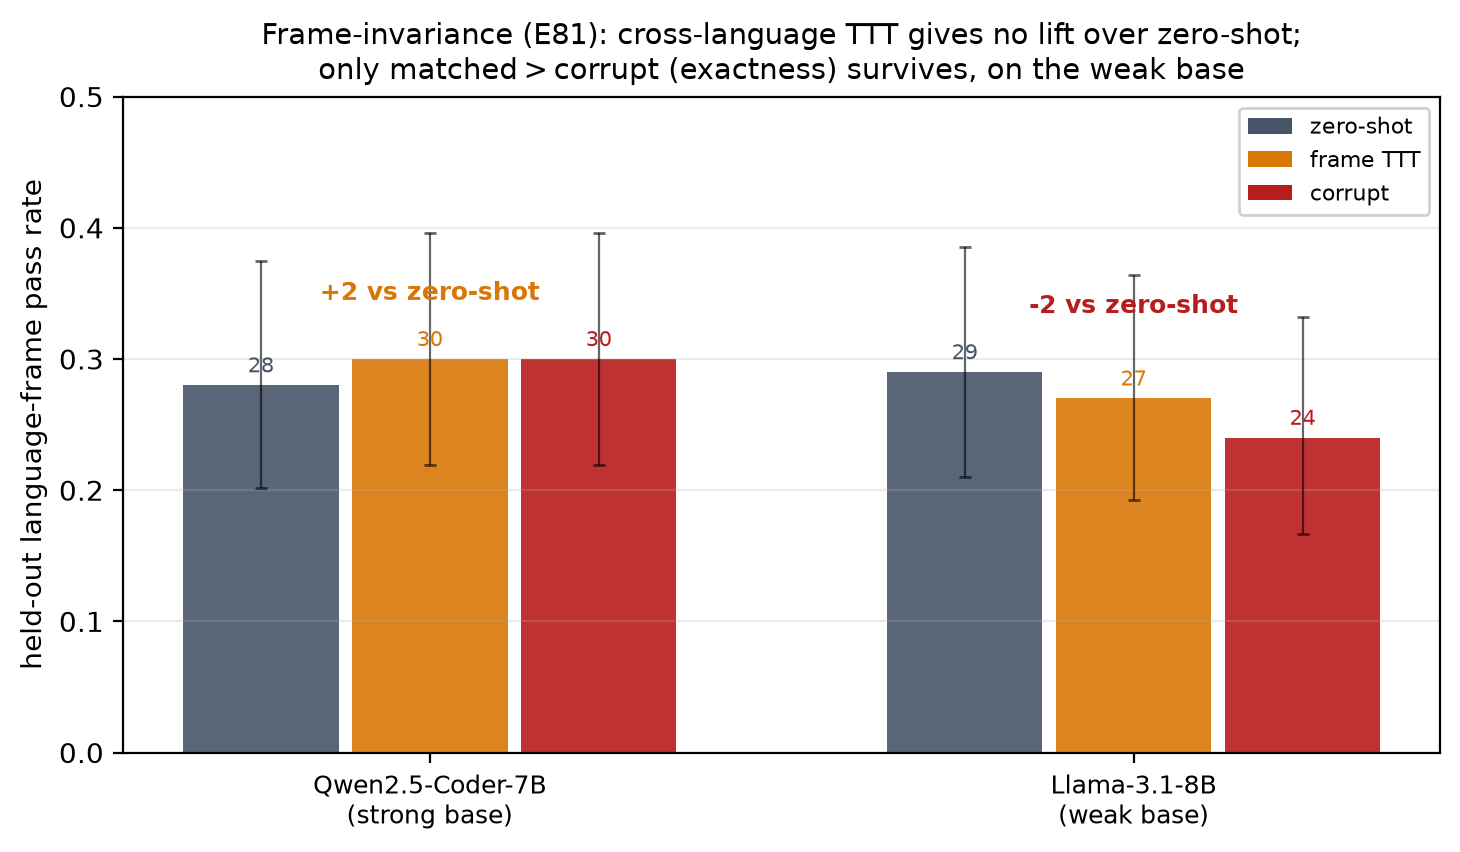
\includegraphics[width=\linewidth,height=0.48\textheight,keepaspectratio]{frame_invariance.png}\vskip3pt{\color{owmuted}\footnotesize Cross-language-frame TTT does not beat zero-shot on either base.\par}
\flushleft \vskip3pt{\footnotesize \begin{itemize}
  \item One problem in 5 languages; train on other frames, test held-out language
  \item Strong coder flat (28\% -> 30\%); weak base drops (29\% -> 27\%)
  \item Only weak exactness ordering survives (matched > corrupt)
  \item A held-out language behaves as its own skill -- an honest boundary
\end{itemize}}
\end{frame}
\begin{frame}{The hybrid loop (E82)}
\centering
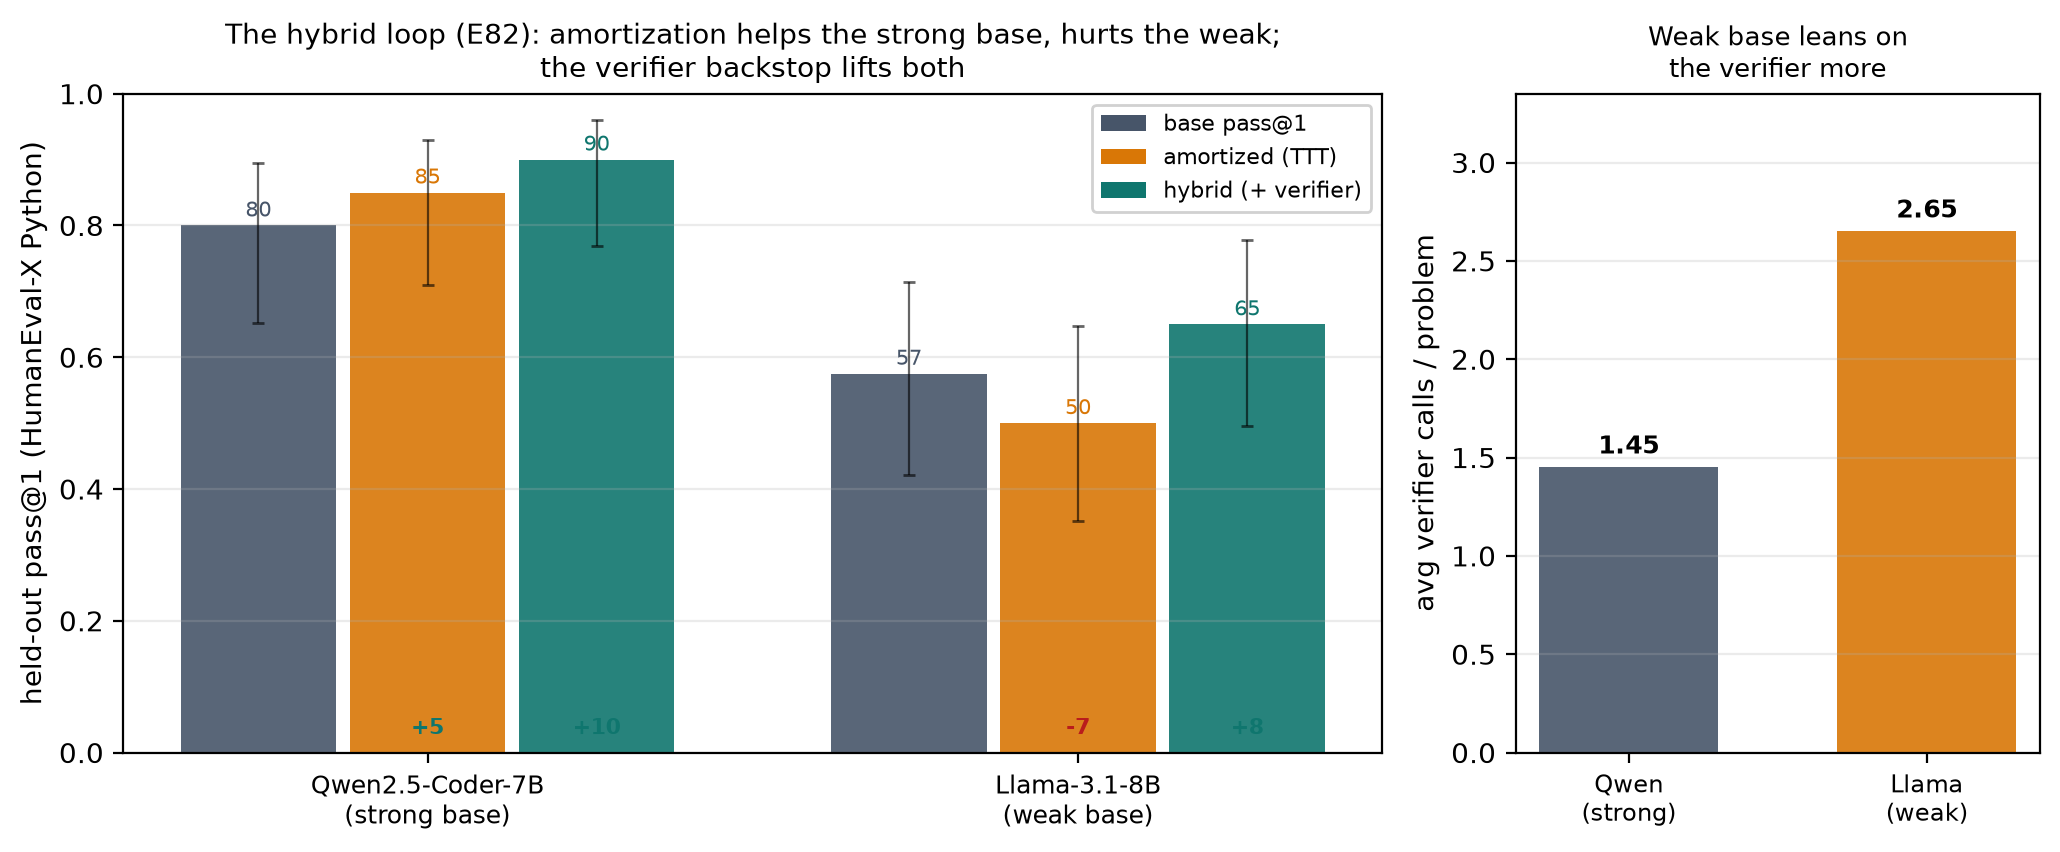
\includegraphics[width=\linewidth,height=0.48\textheight,keepaspectratio]{hybrid_loop.png}\vskip3pt{\color{owmuted}\footnotesize Verified world as generator + verify-and-retry backstop on HumanEval-X.\par}
\flushleft \vskip3pt{\footnotesize \begin{itemize}
  \item Amortization helps strong base (80\% -> 85\%) but hurts weak one (57\% -> 50\%)
  \item Hybrid loop lifts both above base: Qwen 90\% (+10), Llama 65\% (+8)
  \item Weak base leans on the verifier more (2.65 vs 1.45 calls/problem)
  \item Exactness used as an oracle is sufficient -- the robust default route
\end{itemize}}
\end{frame}
\begin{frame}[plain]\centering\vfill
{\color{owochre}\rule{40pt}{2.5pt}}\par\vskip10pt
{\color{owdeep}\bfseries\Large Against Trained \& Perceptual Dynamics\par}\vfill\end{frame}
\begin{frame}{Trained baselines vs zero-transition program (E12)}
\centering

\includegraphics[width=\linewidth,height=0.48\textheight,keepaspectratio]{learned.png}\vskip3pt{\color{owmuted}\footnotesize MLP/1-NN trained on K transitions; none transfers out of distribution.\par}
\flushleft \vskip3pt{\footnotesize \begin{itemize}
  \item At K=10,000 the MLP reaches only 50\% in-dist, 0\% at 10x OOD
  \item Synthesized program: 100\% on both from zero transitions
  \item 1-NN memorizes rollouts (8/8) yet scores 30\% on branch probes
  \item OOD + branch-covering probes, not rollout agreement, measure quality
\end{itemize}}
\end{frame}
\begin{frame}{Induction does not scale with capability (E38)}
\centering

\includegraphics[width=\linewidth,height=0.48\textheight,keepaspectratio]{induction_scale.png}\vskip3pt{\color{owmuted}\footnotesize Trace-induction probe accuracy flat across three generator families.\par}
\flushleft \vskip3pt{\footnotesize \begin{itemize}
  \item From traces alone (no rule text): 0.43 (7B), 0.33 (30B coder), 0.43 (gpt-oss)
  \item None approaches the rule-text anchor of 1.00
  \item Every model exactly scale-invariant (in-dist = 10x OOD)
  \item An identifiability limit of the data, not a capability limit
\end{itemize}}
\end{frame}
\begin{frame}{Acting closes the gap scale cannot (E43)}
\centering

\includegraphics[width=\linewidth,height=0.48\textheight,keepaspectratio]{active_induction.png}\vskip3pt{\color{owmuted}\footnotesize Active version-space elimination beats passive observation.\par}
\flushleft \vskip3pt{\footnotesize \begin{itemize}
  \item Active policy identifies the exact rule in 11.2 transitions vs 14.7 passive
  \item Passive never resolves 2/5 high-k rules within budget
  \item Active (knowing nothing) matches clairvoyant reference (11.2 vs 11.6)
  \item When traces underdetermine dynamics, choose the transitions
\end{itemize}}
\end{frame}
\begin{frame}{The complexity cliff (E20)}
\centering
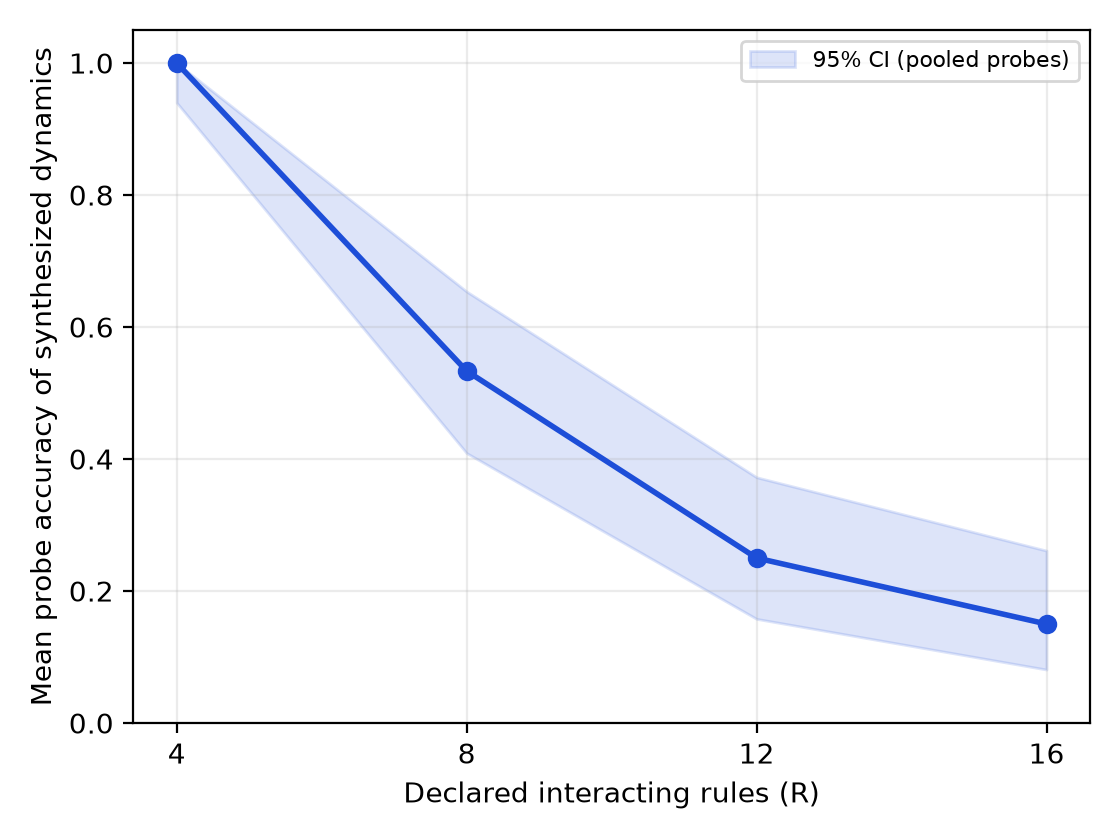
\includegraphics[width=\linewidth,height=0.48\textheight,keepaspectratio]{complexity.png}\vskip3pt{\color{owmuted}\footnotesize Synthesis accuracy vs number of declared interacting rules.\par}
\flushleft \vskip3pt{\footnotesize \begin{itemize}
  \item R=4: 1.00; R=8: 0.53; R=12: 0.25; R=16: 0.15
  \item Monolithic 7B synthesis unreliable past \textasciitilde{}8 coupled rules
  \item The paradigm's present boundary at this model scale
  \item Motivates compositional synthesis -- one expert per rule
\end{itemize}}
\end{frame}
\begin{frame}[plain]\centering\vfill
{\color{owochre}\rule{40pt}{2.5pt}}\par\vskip10pt
{\color{owdeep}\bfseries\Large From Fidelity to Decisions\par}\vfill\end{frame}
\begin{frame}{Planning through a verified world (E22)}
\begin{itemize}
  \item Model-predictive depth-3 lookahead, best action executed in ground truth
  \item Planning through verified program scores 7.5 -- identical to the oracle
  \item Reactive heuristic 5.0; random 3.8; whole episode planned in 0.03 s
  \item Planning through the LLM engine scores 0.0 -- worse than no model
\end{itemize}
\end{frame}
\begin{frame}{Crossing species: bake-off (E63/E65/E67)}
\begin{itemize}
  \item 6 runnable models x 2 symbolic domains: verified code exact and optimal
  \item Every learned model collapses to 0\% exact at 10x OOD
  \item MiniGrid DoorKey: OpenWorld solves zero-shot in an 11-step plan
  \item DreamerV3 needs \textasciitilde{}9,640 interactions to first solve; V-JEPA-2 cannot control
\end{itemize}
\end{frame}
\begin{frame}[plain]\vfill\centering \resizebox{0.95\textwidth}{!}{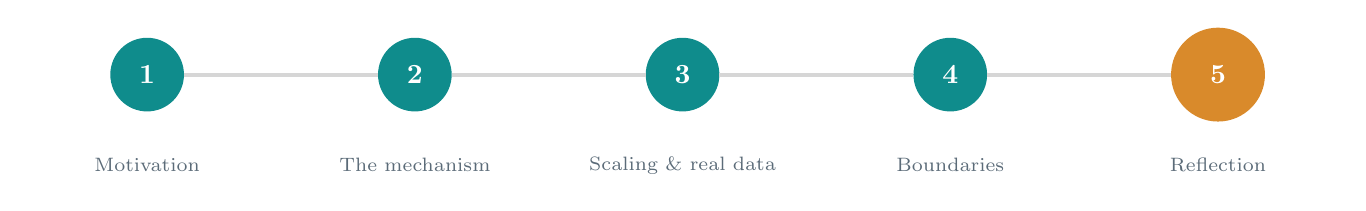
\begin{tikzpicture}[stn/.style={circle,draw=owteal,line width=1pt,minimum size=9mm,font=\bfseries,inner sep=0,text=owteal},std/.style={circle,draw=owteal,fill=owteal,line width=1pt,minimum size=9mm,font=\bfseries,inner sep=0,text=white},stc/.style={circle,draw=owochre,fill=owochre,line width=1.2pt,minimum size=11.5mm,font=\bfseries,inner sep=0,text=white},stx/.style={circle,draw=owmuted,line width=1pt,minimum size=9mm,font=\bfseries,inner sep=0,text=owmuted},stlbl/.style={font=\scriptsize,text=owmuted,align=center,text width=28mm},stln/.style={draw=black!16,line width=1.4pt}]\node[std] (s0) at (0.0,0) {1};\node[std] (s1) at (3.4,0) {2};\node[std] (s2) at (6.8,0) {3};\node[std] (s3) at (10.2,0) {4};\node[stc] (s4) at (13.6,0) {5};\node[stlbl] at (0.0,-1.15) {Motivation};\node[stlbl] at (3.4,-1.15) {The mechanism};\node[stlbl] at (6.8,-1.15) {Scaling \& real data};\node[stlbl] at (10.2,-1.15) {Boundaries};\node[stlbl] at (13.6,-1.15) {Reflection};\draw[stln] (s0)--(s1);\draw[stln] (s1)--(s2);\draw[stln] (s2)--(s3);\draw[stln] (s3)--(s4);\end{tikzpicture}}\\[24pt]
{\color{owochre}\bfseries\footnotesize PART 5}\\[5pt]
{\color{owdeep}\bfseries\Large Reflection}\\[10pt]{\color{owmuted}\large Discussion, limitations, conclusion}\vfill\end{frame}
\begin{frame}{Is world-time compute just fine-tuning?}
\begin{itemize}
  \item Mechanically yes -- LoRA-SFT; the claim is about the data source
  \item A correct world model turns compute into unlimited correct training data
  \item Two things earn the name: verified-label dependence and cross-world transfer
  \item Where neither holds, it is fairly just expensive fine-tuning -- and we say so
\end{itemize}
\end{frame}
\begin{frame}{The trajectory unit, measured (E85)}
\begin{itemize}
  \item Training unit is a transition (s,a,s'), not a final answer
  \item At the trained horizon: trajectory 70\% vs answer 58\% (+12 pts)
  \item Rolled out longer than trained, answer unit catches up (75\% vs 68\%)
  \item Composing per-step predictions reintroduces compounding on the learned side
\end{itemize}
\end{frame}
\begin{frame}{When does it pay off? Few-step reasoning}
\begin{itemize}
  \item Wins where a task is few steps over state that can be told symbolically
  \item Shallow rule induction, small grid transforms, short-horizon planning
  \item Degrades as reasoning lengthens (CLRS traces, >8 composed rules)
  \item Cedes long-horizon, perception-heavy regimes to learned models
\end{itemize}
\end{frame}
\begin{frame}{Three routes to use a verified world model}\vfill\begin{columns}[T]\begin{column}{0.237\textwidth}{\color{owteal}\rule{20pt}{3pt}}\par\smallskip{\color{owdeep}\bfseries Tool}\par\smallskip{\small Serve, plan, verify — no training}\end{column}\begin{column}{0.237\textwidth}{\color{owochre}\rule{20pt}{3pt}}\par\smallskip{\color{owdeep}\bfseries Per-world TTT}\par\smallskip{\small Distill one world's trajectories}\end{column}\begin{column}{0.237\textwidth}{\color{owblue}\rule{20pt}{3pt}}\par\smallskip{\color{owdeep}\bfseries World-time compute}\par\smallskip{\small Traverse a family; generalize}\end{column}\begin{column}{0.237\textwidth}{\color{owmuted}\rule{20pt}{3pt}}\par\smallskip{\color{owdeep}\bfseries Hybrid}\par\smallskip{\small Exact data + verify backstop}\end{column}\end{columns}\vfill\end{frame}
\begin{frame}{Limitations}\vfill\begin{columns}[T]\begin{column}{0.237\textwidth}{\color{owteal}\rule{20pt}{3pt}}\par\smallskip{\color{owdeep}\bfseries Scope}\par\smallskip{\small Symbolic, not pixel-native}\end{column}\begin{column}{0.237\textwidth}{\color{owochre}\rule{20pt}{3pt}}\par\smallskip{\color{owdeep}\bfseries Complexity}\par\smallskip{\small Cliff past \textasciitilde{}8 rules}\end{column}\begin{column}{0.237\textwidth}{\color{owblue}\rule{20pt}{3pt}}\par\smallskip{\color{owdeep}\bfseries Variance}\par\smallskip{\small Some numbers single-seed}\end{column}\begin{column}{0.237\textwidth}{\color{owmuted}\rule{20pt}{3pt}}\par\smallskip{\color{owdeep}\bfseries Stats}\par\smallskip{\small No family-wise correction}\end{column}\end{columns}\vfill\end{frame}
\begin{frame}[plain]\centering\vfill
{\color{owochre}\rule{40pt}{2.5pt}}\par\vskip10pt
{\color{owdeep}\bfseries\Large Conclusion\par}\vfill\end{frame}
\begin{frame}[plain]\centering\vfill
{\color{owdeep}\bfseries\LARGE Make the model a program, verify the program, and keep the values dialable -- an orthogonal path to scaling parameters until hallucination is suppressed.\par}\vfill\end{frame}
\begin{frame}{Takeaways}
\begin{itemize}
  \item Verified code world models are bit-exact where learned dynamics compound error
  \item Plan as well as ground truth; hallucinated planning is worse than none
  \item Traversing many verified worlds lifts generalization to held-out worlds
  \item Next: compositional synthesis, benchmark-scale coding, perception-to-symbol pipelines
\end{itemize}
\end{frame}
\end{document}
